\chapter{Einführung}
\section{Beispielanwendung}
Im Zuge der Diplomarbeit soll neben einem Vergleich von Pythonwebframeworks auch
eine Anwendung für des Rechnertechniklabor der HS Augsburg entwickelt werden.
Dabei soll der Zugriff auf Informationen und Verwaltung der Mikrocontroller in
Form einer Webanwendung möglich sein. Dabei kann der Benutzer die einzelnen
Boards reservieren und anschließend per SSH über das Internet mit den Boards
arbeiten können. Damit ein reibungsloser Umgang auf den Boards ermöglicht wird
soll jeweils einem einzelnen Benutzer gleichzeitig der Zugang auf ein Board 
gewährt werden. Darüber hinaus wird folgende Funktionalität von der Andwendung 
aus zugänglich:

\begin{itemize}
  \item Power on/off
  \item Reset
  \item Statusinformationen abrufen
  \item Reservierung
  \item Webupload der Root-Filesysteme
\end{itemize}

Weiterhin bekommt der Benuzter die Möglichkeite Statusinformationen abzurufen, 
die auf der Weboberfläche angezeigt werden. Darüber hinaus auch ein Webupload
von Rootfilesystemen möglich, die auf dem Board mit Hilfe von Skripten auf die
Boards automatisch aufgespielt werden. Zu den Arbeiten gehört weiterhin die
Installation entsprechender Frameworks und nötige Software für den
Reibungslosen Ablauf der Applikation. Die Anwendung wird gegebenenfalls unter
verschiedenen Technologien implementieret. Nach der Reservierung der Boards
bekommt der Benuzter einen Zugang mit Passwort, damit dieser über SSH auf das
Board zugreifen kann. Das Passwort wir nach Reservierung jeweils neu erstellt
und nach dem Abmelden aus der Userverwaltung oder nachdem der User nicht mehr
auf dem Board arbeiten will der Zugang gesperrt, bis ein anderer das Board
reserviert. 

Für jedes der hier vorgestellten Webframeworks wird diese Anwendung entwickelt.
Es soll nach dem Durchlesen dieser Arbeit möglich sein, ein Vergleich zu ziehen,
welches Framework die beste Unterstützung bietet, um Webprojekte im
Pythomumfeld zu erstellen. Normalerweise denkt man heutzutage bei
Webentwicklung hauptsächlich an \emph{PHP} als Hauptsprache, für die es
unzählige Frameworks und Anwendungen\footnote{\url{magentocommerce.com},
\url{atmail.com}} gibt. Auch wird oft \emph{Ruby on Rails} im Zusammenhang
gebracht, bei der es eine große Entwicklergemeinde existiert und ebensoviele 
bekannte Projekte\footnote{unter anderen \url{twitter.com}, \url{shopify.com}, 
\url{github.com}}.

So soll aufgezeigt werden, dass auch der Pythonentwickler seine hart erarbeiten
Kenntnisse auch im Webumfeld einsetzen kann und keine neue Programmiersprache
dafür lernen muss. Mit Django, ZOPE, Pylons, web2py gibt es genug Alternativen
für die Entwicklungen von Anwendungen in der Python-Welt. Diese werden anhand
einer Beispielanwendung vorgestellt und untersucht.

\section{Durchführung}
\subsection{GUI}
Da es sich um eine Webanwendung handelt, kommen für die Interaktion des
Benutzers mit der Schnittselle XHTML\footnote{XHTML: Extensible
HyperText Markup Language, \url{http://www.w3.org/TR/xhtml1/} } für die
Struktur und den Inhalt, CSS2\footnote{Cascading Stylesheets  Level 2,
\url{http://www.edition-w3.de/TR/1998/REC-CSS2-19980512/}} für die Gestaltung 
und JavaScript auch in Form eines Frameworks, abhänging davon, was das 
Webframework anbietet, in Frage. Beispiele für
JavaScript-Frameworks\footnote{JavaScript-Frameworks:
\url{http://webstandard.kulando.de/post/2008/08/21/top-10-aller-javascript-
frameworks}} sind z.B. jQuery, Dojo oder Prototype mit denen eine Vereinfachte
Interaktion mit dem Benutzer erstellt werden kann. Da diese Frameworks die
Möglichkeit bieten AJAX \footnote{AJAX: Asynchronous 
Javascript and XML,
\url{http://openbook.galileocomputing.de/javascript_ajax/18_ajax_001.htm}}
Funktionalität anzuwenden, kann eine Resourcen schonende Applikation mit
schnellen Reaktionszeiten erstellt werden, da nicht alle Teile der Anwendung 
geladen werden müssen.

Auf folgender Vorlage\ref{guianwendung}, die mittels HMTL und CSS erstellt
worden ist, basiert die GUI der Anwendung. Es wurde durchgehend darauf
geachtet,  dass \emph{em} als Maßeinheit verwendet wird, um ein
elastisches\footnote{\url{http://greattalk.ch/2008/02/09/die-unglaublichen-em-
elastischen-layouts-mit-css/}} Layout sicherzustellen. Der Vorteil liegt hier 
in der besseren Zugänglichkeite der Seite und der Anpassung des Designs an die 
Schriftgröße des Browsers, welche der User benutzt. So bleiben Skalierungen 
proportional und es entstehen weniger negative Seiteneffekte beim Zoomen der
Seite.

\begin{figure}[ht]
 \begin{center}
  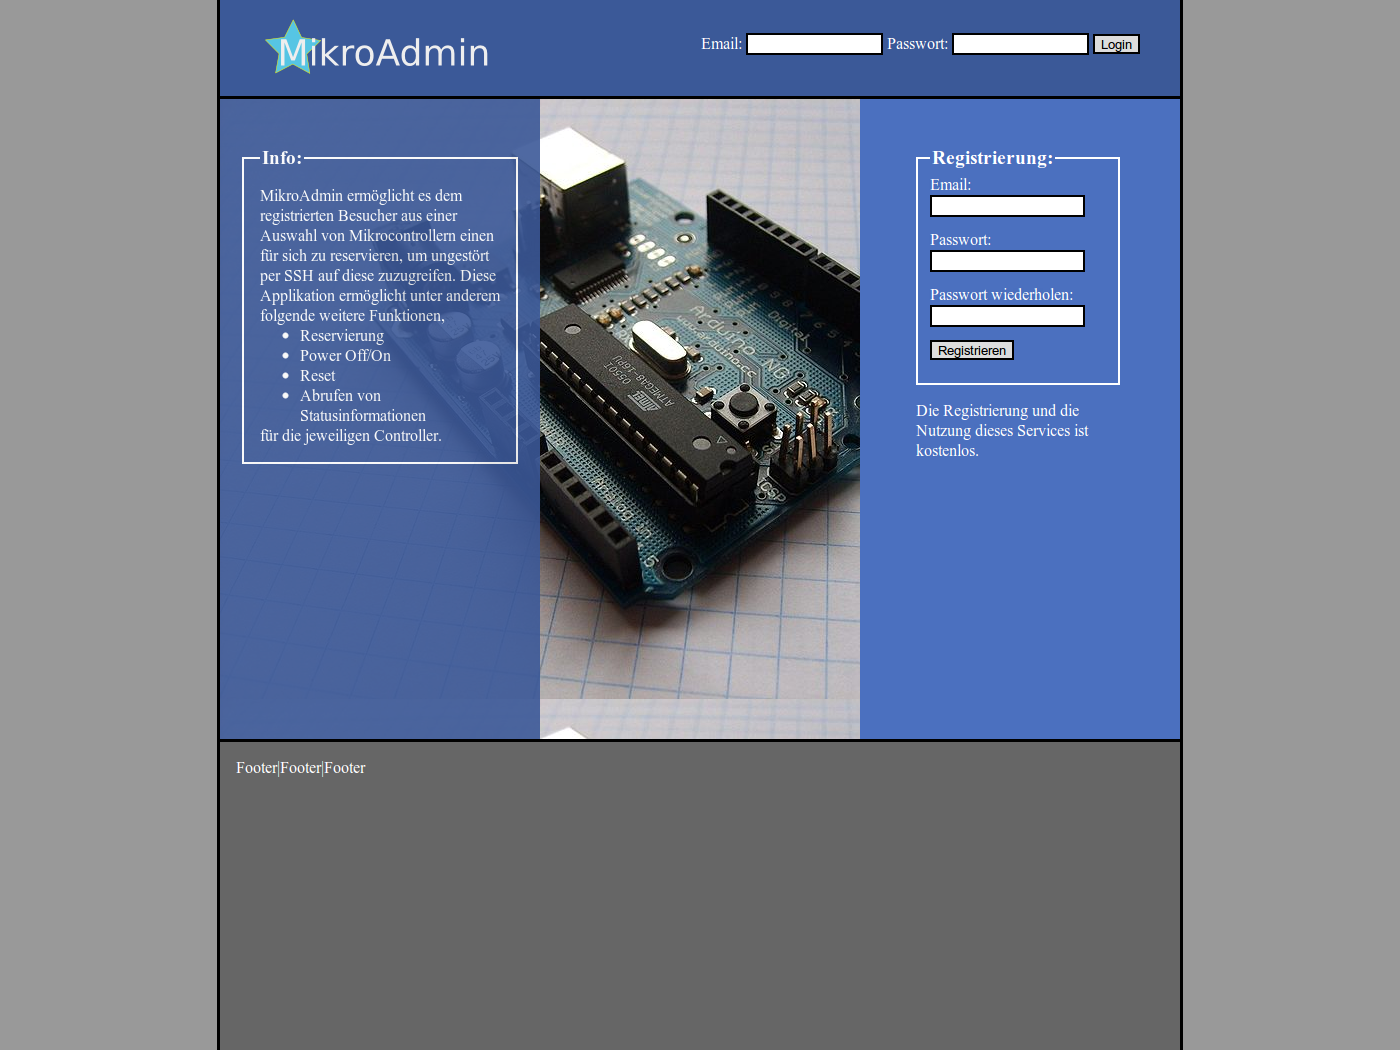
\includegraphics[scale=0.25]{/home/jupiter/andres/programmieren/latex/eclipseLatexWorkspaceNew/latex/diplomarbeit/images/gui.png}
 \end{center}
 \caption{GUI der Anwendung}
 \label{guianwendung}
\end{figure}

Darauf aufbauend, wird das Template in den jeweiligen Frameworks angepasst und
weitere Unterseiten von dieser Seite so weit es geht abgeleitet. So wird es
einfacher die jeweiligen Möglichkeiten der Template Sprachen der verschiedenen
Frameworks zu vergleichen. Der Code des Templates kann unter folgender Adresse
eingesehen werden.


\subsection{Datenbank}
\subsection{Logik}